\documentclass[11pt,a4paper]{article}
\usepackage[margin=2.5cm]{geometry}
\usepackage{graphicx}
\usepackage{amsmath}
\usepackage{hyperref}
\newcommand{\un}[2]{\ensuremath{#1\,\mathrm{#2}}}

\title{AC-DC Boost PFC vs.\ DC-DC Boost Converter:\\
       Ripple, Input Current and Startup Comparison}
\author{Aayush Singh\\ Department of Electrical and Electronics Engineering, NIT Goa}
\date{\today}

\begin{document}
\maketitle

\begin{abstract}
A single-phase AC-DC boost converter with power-factor correction (PFC) is compared
against a plain DC-DC boost converter of identical power stage and control, both
regulating $415\,\mathrm{V}$ into a $100\,\Omega$ load at $f_{sw}=1\,\mathrm{kHz}$ in Simulink.
The DC converter shows about $12\times$ lower output voltage ripple, while the AC-DC
converter draws a line-following input current with $8.9\,\%$ THD and a power factor of
$0.995$. The $100\,\mathrm{Hz}$ ripple of the AC-DC converter agrees with the analytical
estimate. A startup study shows that clamping anti-windup on the PI controllers removes
the output overshoot and cuts the settling time from over a second to under half a second.
\end{abstract}

\section{Introduction}
A boost converter fed from a rectified AC line must shape its input current to follow
the line voltage, otherwise it draws distorted, low-power-factor current. The price is a
pulsating power flow at twice the line frequency, which appears as low-frequency ripple
on the output. This report quantifies that trade-off by simulating, side by side and with
identical controllers, (i) a boost PFC fed from a rectified $230\,\mathrm{V}$ peak,
$50\,\mathrm{Hz}$ source and (ii) a boost converter fed from a DC source of equal average
input voltage. Metrics compared are output ripple, input current, THD and power factor,
and startup behaviour.

\section{Simulation Setup}
Both converters sit in one Simulink/Simscape Electrical model with shared scopes
(discrete solver, $10\,\mu\mathrm{s}$ step). The circuit is shown in Fig.~\ref{fig:circuit};
the only intended difference is the source.

\begin{table}[htbp]
\centering
\begin{tabular}{|l|l|}
\hline
Parameter & Value \\ \hline
Boost inductor $L$ & $5\,\mathrm{mH}$ \\
Output capacitor $C$ & $10\,\mathrm{mF}$ \\
Load $R$ & $100\,\Omega$ ($\approx1.72\,\mathrm{kW}$ at $415\,\mathrm{V}$) \\
Switching frequency $f_{sw}$ & $1\,\mathrm{kHz}$ (PWM period $10^{-3}\,\mathrm{s}$) \\
Output reference & $415\,\mathrm{V}$ \\
AC source (AC-DC bench) & $230\,\mathrm{V}$ peak, $50\,\mathrm{Hz}$, through a diode bridge \\
DC source (DC bench) & $146\,\mathrm{V}$ ($=2\cdot230/\pi$, average of rectified AC) \\
Outer voltage PI & $P=0.005$, $I=0.05$; output limited to $0$--$0.15$ \\
Inner current PI & $P=0.5$, $I=100$; output (duty) limited to $0$--$0.95$ \\
Anti-windup & clamping, on both PI stages \\ \hline
\end{tabular}
\caption{Common parameters of both benches.}
\end{table}

\begin{figure}[htbp]
\centering
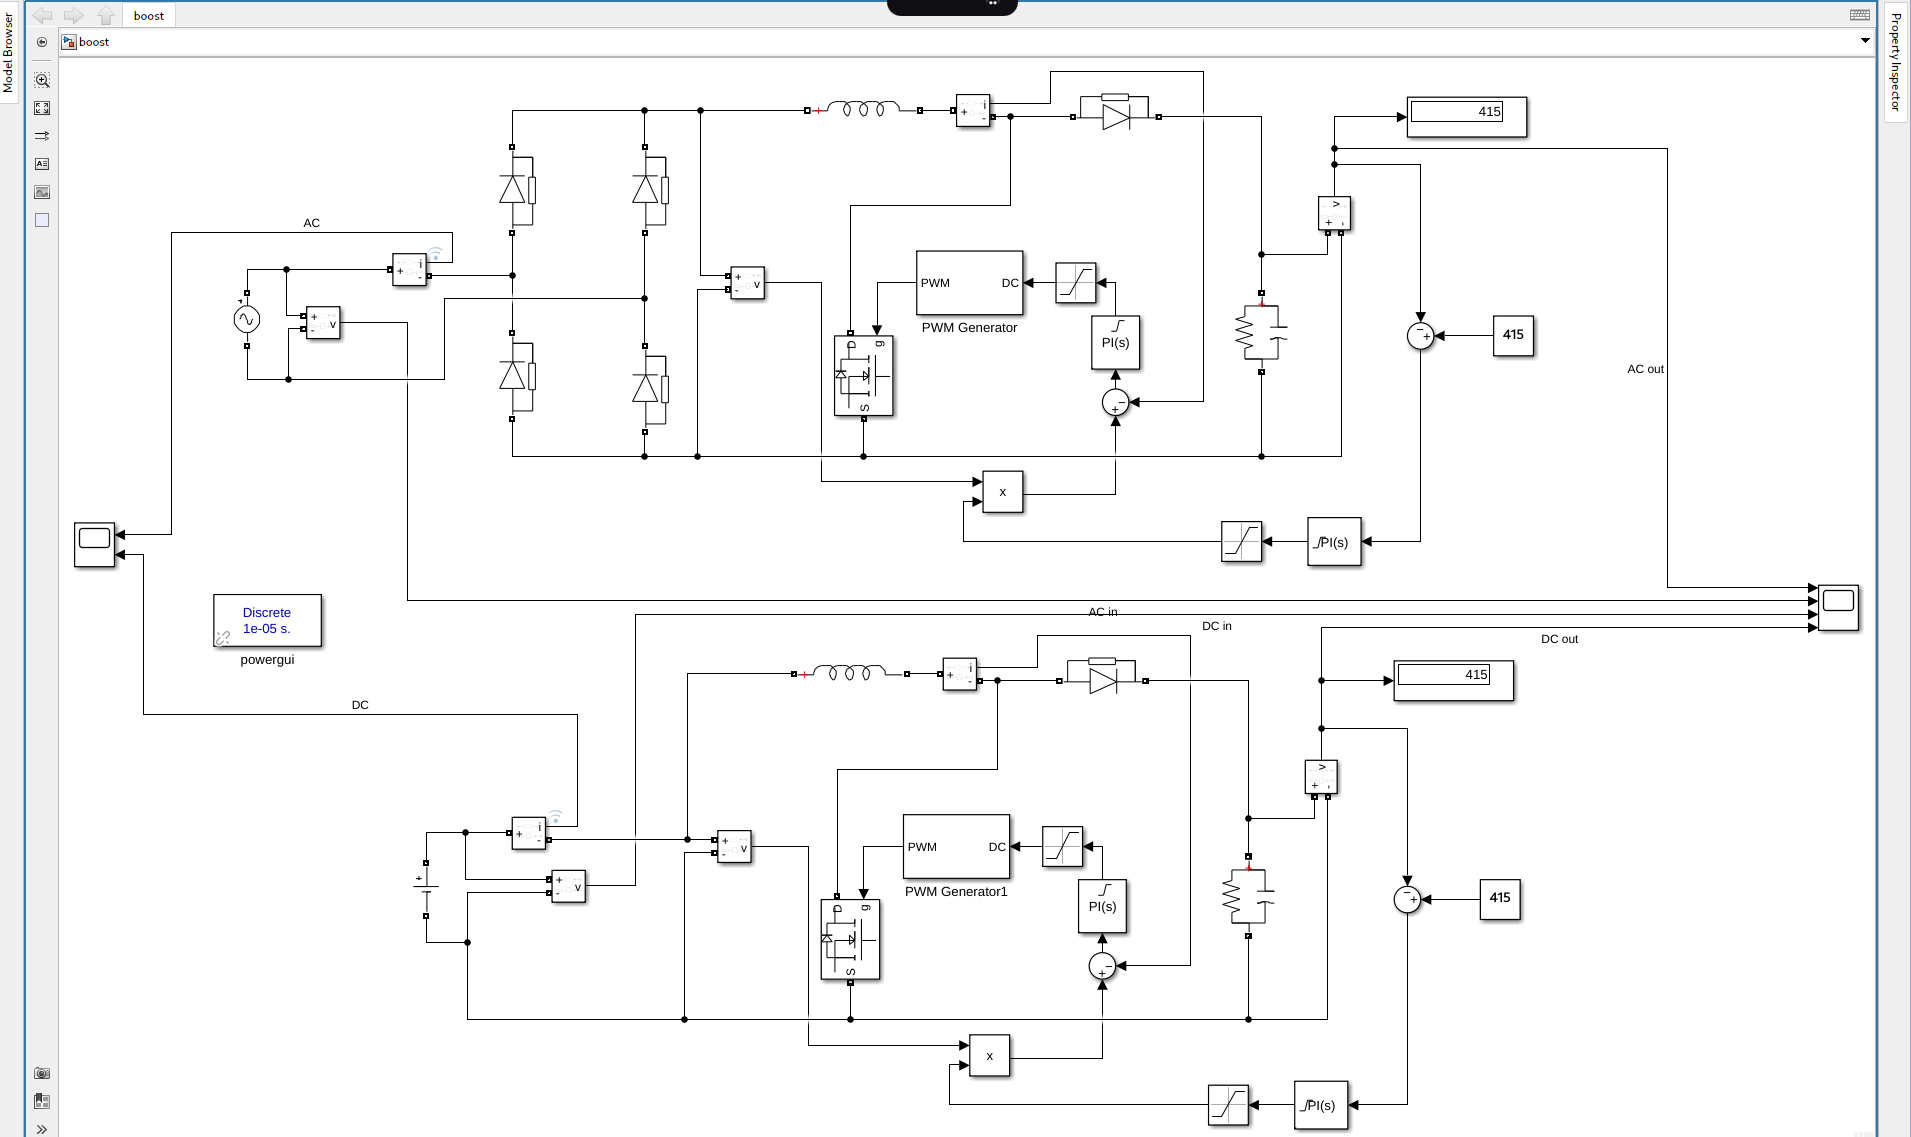
\includegraphics[width=0.92\linewidth]{circuit.png}
\caption{Boost converter simulation circuit used for the AC-DC and DC-DC comparison.}
\label{fig:circuit}
\end{figure}

\paragraph{Control structure.} An outer voltage PI acts on the error between the $415\,\mathrm{V}$
reference and the output voltage. Its output is multiplied by the (rectified) input voltage to
form the inductor-current reference, so the commanded current follows the input voltage shape.
An inner PI acts on the current error and sets the PWM duty cycle. The DC bench uses the same
structure with a constant input voltage.

\paragraph{Fair comparison.} The DC source equals the average of the rectified AC input
($146\,\mathrm{V}$), and both benches deliver the same output power, so the mean input
current of the DC bench ($\approx12\,\mathrm{A}$) matches $P_o/V_{in}=1722/146\approx11.8\,\mathrm{A}$.
The inductor current of the DC bench never reaches zero, i.e.\ it operates in continuous conduction.

\paragraph{Measurement windows.} Output ripple was evaluated over $0.8$--$1.0\,\mathrm{s}$
(ten line cycles); THD and power factor over $0.6$--$1.0\,\mathrm{s}$ (twenty line cycles).
Switching ripple is the peak-to-peak of the output voltage after removing a $1\,\mathrm{ms}$
moving average. THD includes harmonics up to the 40th ($2\,\mathrm{kHz}$).

\section{Controller Development: Startup and Anti-Windup}
Four configurations were simulated in sequence. Values are read from the scope plots and are
approximate.

\begin{table}[htbp]
\centering
\small
\begin{tabular}{|p{3.2cm}|p{2.4cm}|p{2.6cm}|p{4.8cm}|}
\hline
Configuration & Overshoot (AC-DC / DC) & Settling to $\pm1\,\%$ (AC-DC / DC) & Remark \\ \hline
A: DC source $207\,\mathrm{V}$, limits ineffective ($0$--$600$) &
$480\,\mathrm{V}$ / $705\,\mathrm{V}$ & $0.35\,\mathrm{s}$ / $1.4\,\mathrm{s}$ &
DC output decays to $\approx237\,\mathrm{V}$ before recovering \\ \hline
B: DC source $146\,\mathrm{V}$, limits ineffective &
$480\,\mathrm{V}$ / $508\,\mathrm{V}$ & $0.4\,\mathrm{s}$ / $0.6\,\mathrm{s}$ &
DC undershoot to $\approx373\,\mathrm{V}$ (integrator windup) \\ \hline
C: limits as separate saturation blocks only &
$515\,\mathrm{V}$ / $508\,\mathrm{V}$ & $0.85\,\mathrm{s}$ / $1.2\,\mathrm{s}$ &
Current held at its limit $\approx0.25$--$0.5\,\mathrm{s}$ past $415\,\mathrm{V}$ \\ \hline
D: limits inside PI blocks, clamping anti-windup &
none & $0.4\,\mathrm{s}$ / $0.45\,\mathrm{s}$ &
Final design used for all other results \\ \hline
\end{tabular}
\caption{Effect of source level, current limits and anti-windup on startup.}
\end{table}

The slow decline of the DC output after the overshoot in A and B is the output capacitor
discharging into the load ($RC=1\,\mathrm{s}$): a boost converter cannot pull its output down, so
once the integrator has wound up the output only falls through the load. Setting the output
limits and the anti-windup method inside the PI blocks lets the integrator back off as soon
as the error changes sign (D).

\section{Results}
All results below are for configuration D.

\subsection{Startup}
Figures~\ref{fig:startv} and \ref{fig:startc} show the first second. Before the controller acts,
the input source charges the output capacitor through the inductor and the boost diode, giving a
passive LC inrush $I_{pk}\approx V_{in}\sqrt{C/L}\approx206\,\mathrm{A}$ and an output of about
$2V_{in}\approx290\,\mathrm{V}$ (measured: $293\,\mathrm{V}$ AC-DC, $289\,\mathrm{V}$ DC; current
peaks of $\approx225\,\mathrm{A}$ and $205\,\mathrm{A}$). The output then dips (to $\approx271\,\mathrm{V}$
and $259\,\mathrm{V}$) while the capacitor discharges into the load before switching begins
(at $\approx0.10\,\mathrm{s}$ and $0.13\,\mathrm{s}$). The current then sits at its limit
($22\,\mathrm{A}$ DC, $\approx36\,\mathrm{A}$ peak AC), and relaxes to steady state as the output
approaches $415\,\mathrm{V}$ without overshoot.

\begin{figure}[htbp]
  \centering
  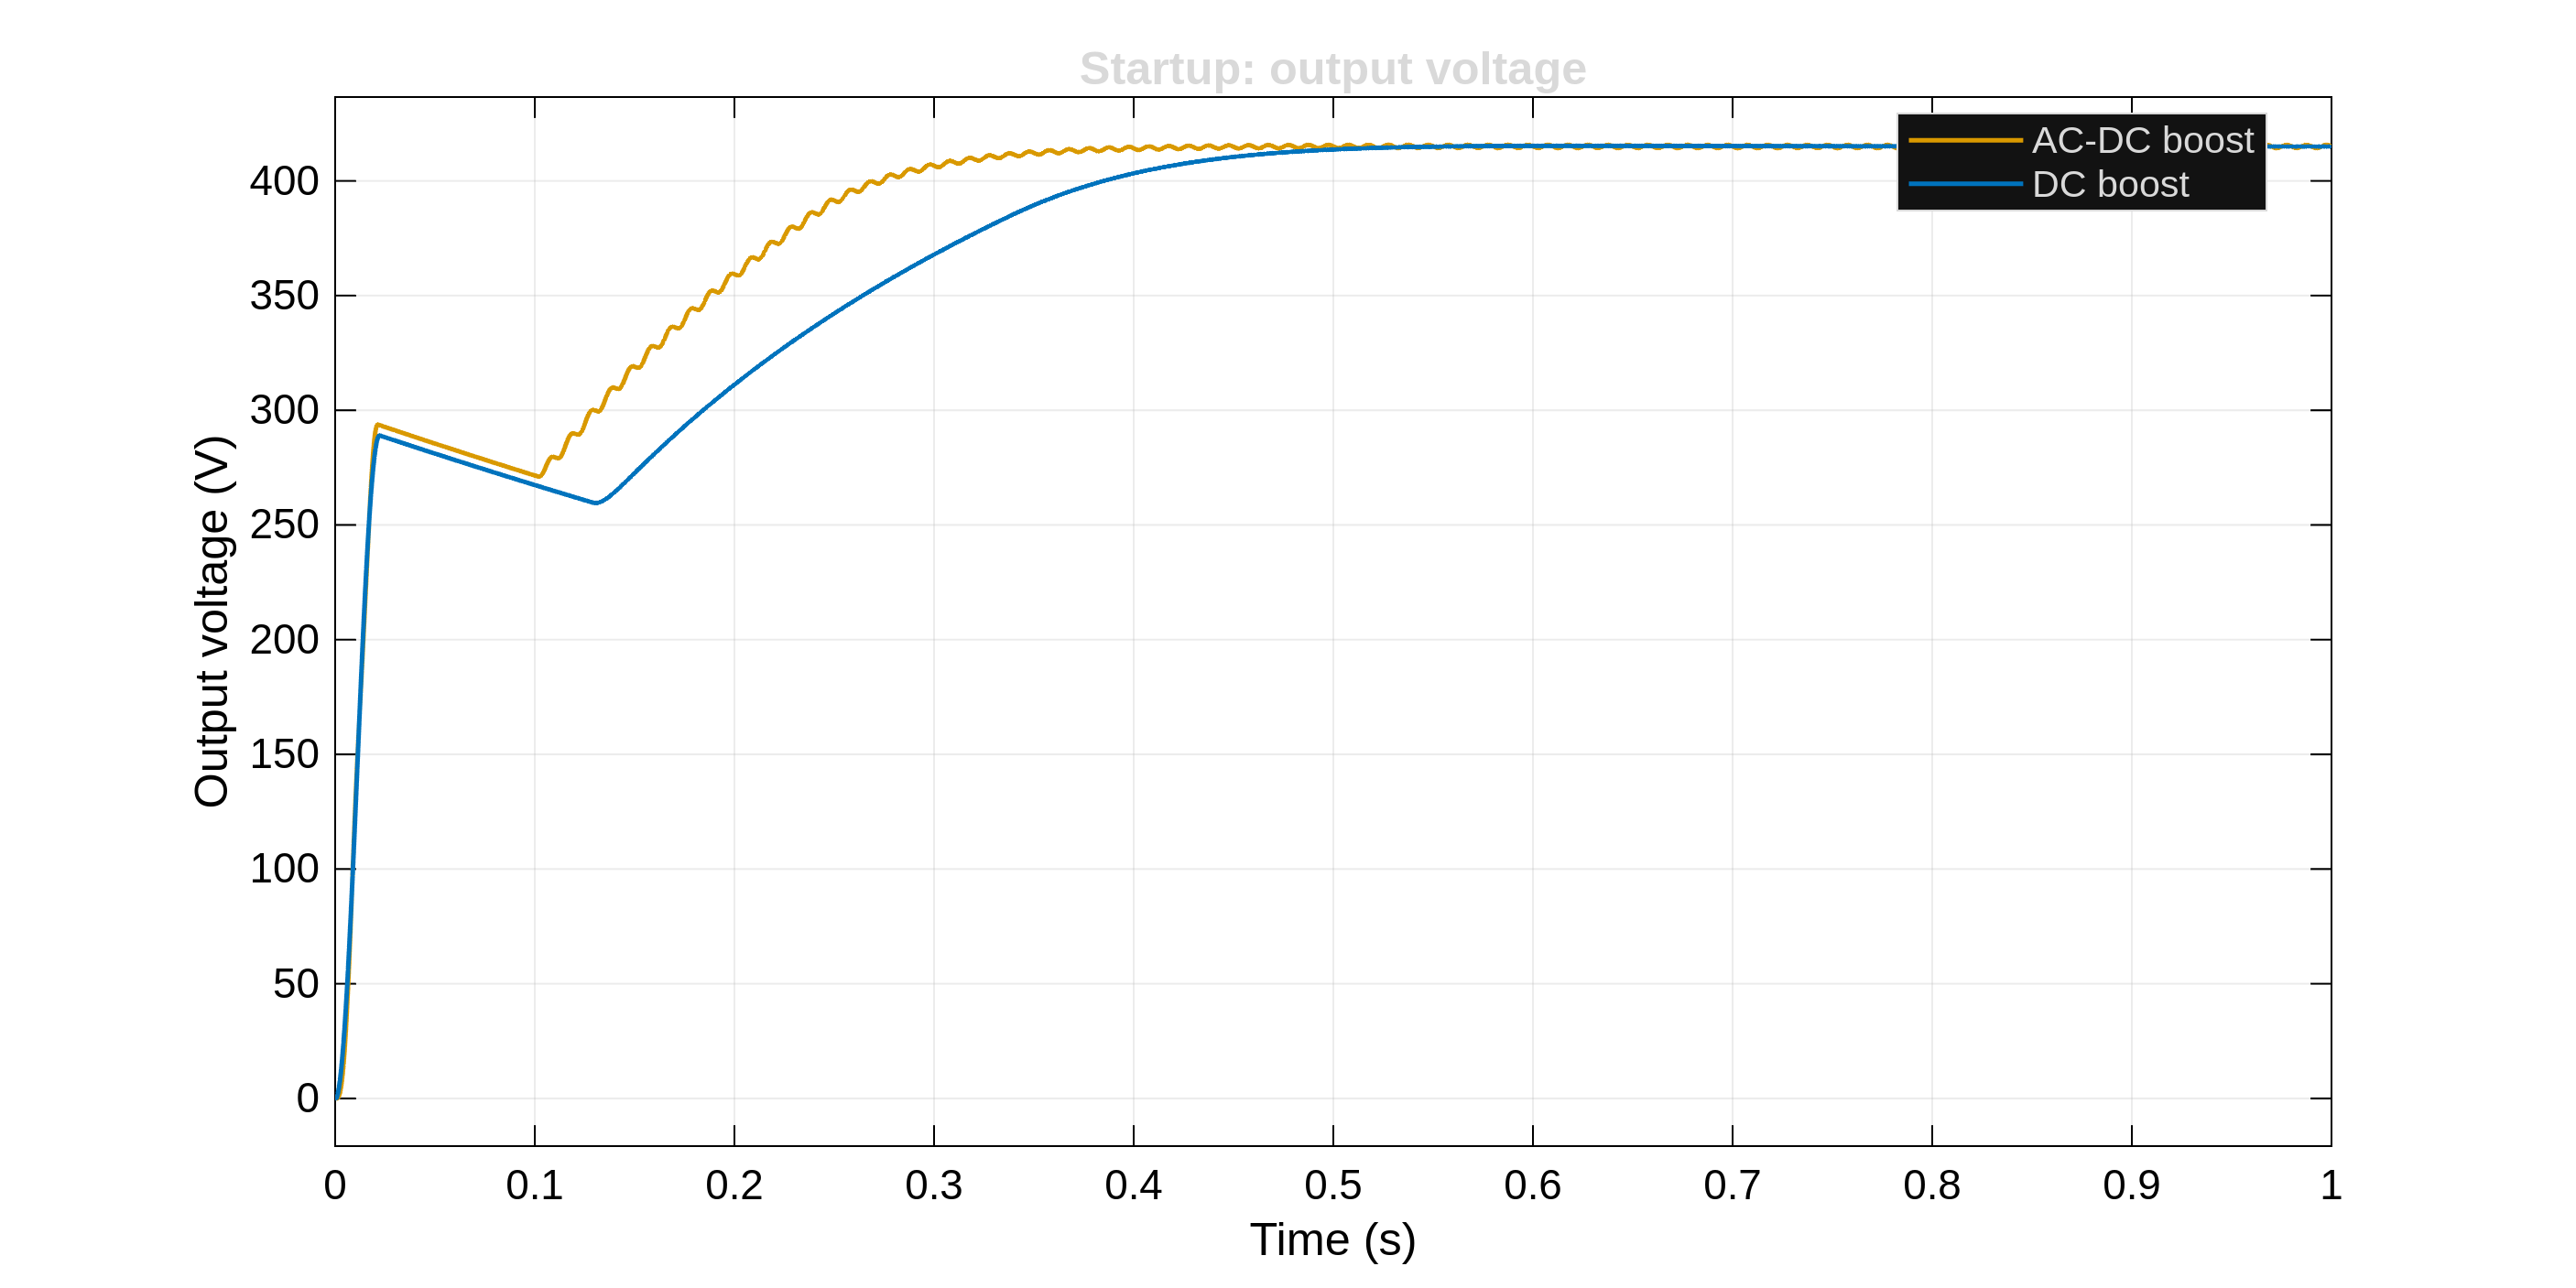
\includegraphics[width=0.92\linewidth]{fig_startup_voltage.png}
  \caption{Startup output voltage of the AC-DC and DC boost converters.}
  \label{fig:startv}
\end{figure}

\begin{figure}[htbp]
  \centering
  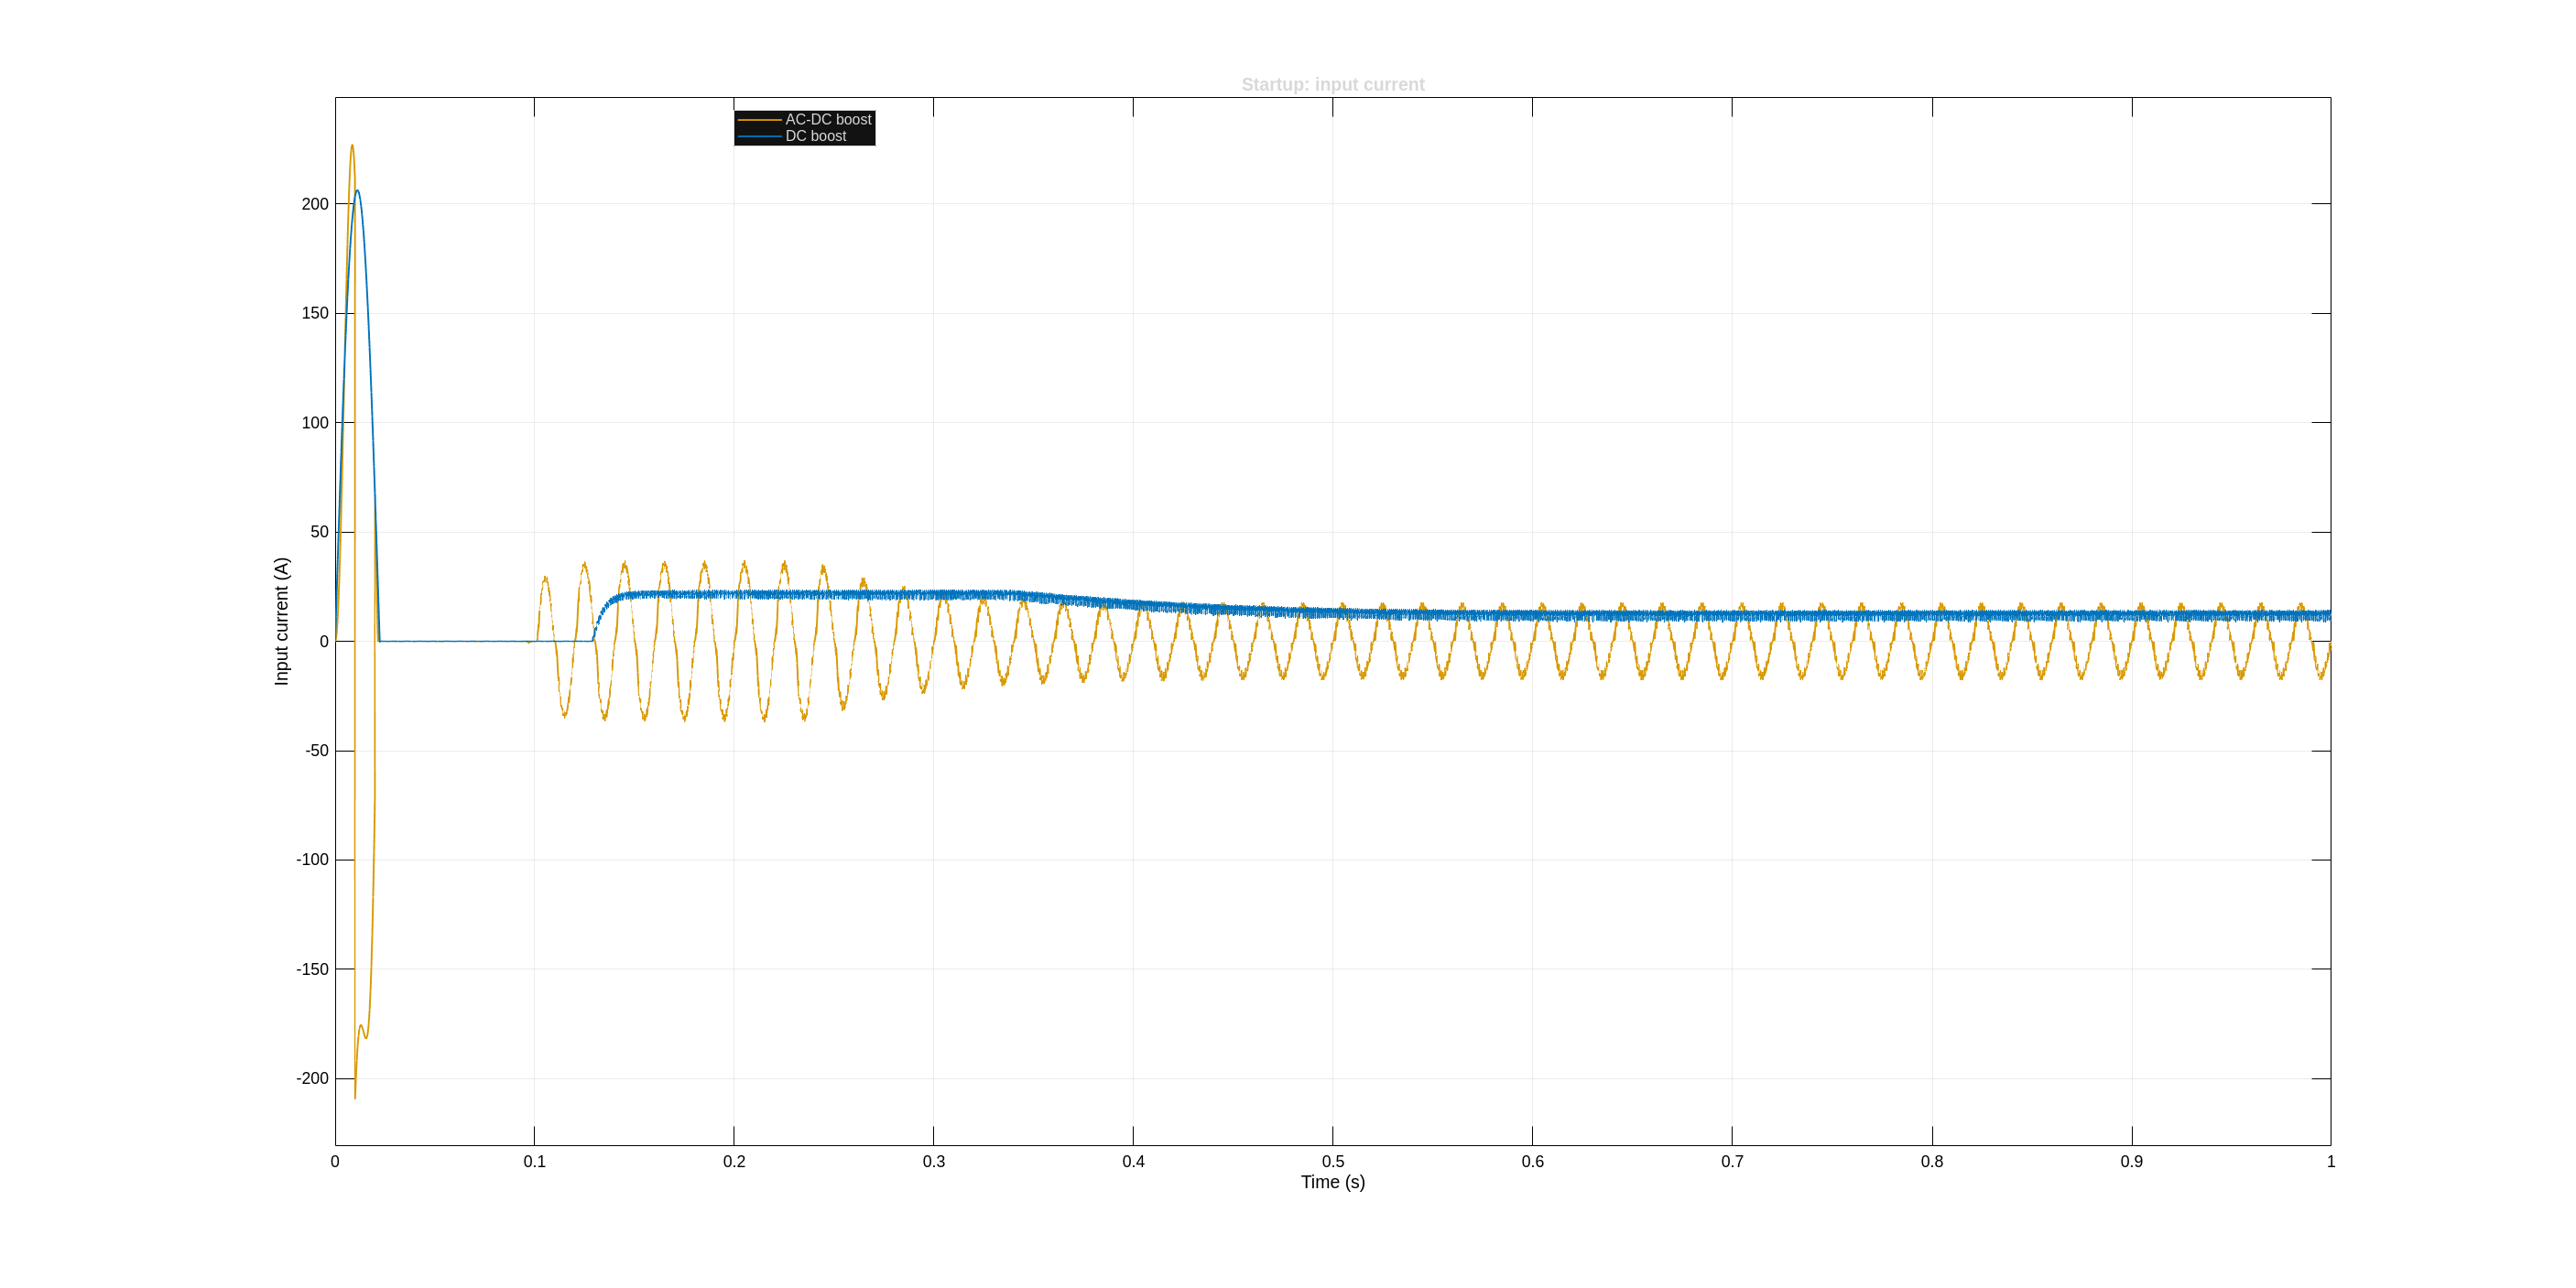
\includegraphics[width=0.92\linewidth]{fig_startup_current.png}
  \caption{Startup input current. The initial spike is the passive LC inrush; the plateau is the
  current limit.}
  \label{fig:startc}
\end{figure}

\subsection{Output Voltage Ripple}
\begin{table}[htbp]
\centering
\begin{tabular}{|l|c|c|}
\hline
Quantity & AC-DC boost & DC boost \\ \hline
Output ripple, total pk-pk & $1.45\,\mathrm{V}$ ($0.35\,\%$) & $0.12\,\mathrm{V}$ ($0.03\,\%$) \\ \hline
Switching ripple ($1\,\mathrm{kHz}$) pk-pk & $0.15\,\mathrm{V}$ & $0.075\,\mathrm{V}$ \\ \hline
$100\,\mathrm{Hz}$ component pk-pk & $\approx1.3\,\mathrm{V}$ & none \\ \hline
\end{tabular}
\caption{Steady-state output ripple. The DC total includes about $0.05\,\mathrm{V}$ of residual
drift towards $415\,\mathrm{V}$ inside the window; its switching ripple is the representative figure.}
\end{table}

With constant load power and an input power that pulsates at $2f_{line}$, the output capacitor
must absorb the difference. The resulting ripple is
\[
\Delta V_{pp}\approx\frac{P_o}{2\pi f_{line}\,C\,V_o}
=\frac{1722}{2\pi\cdot50\cdot0.01\cdot415}\approx1.32\,\mathrm{V},
\]
in good agreement with the measured $\approx1.3\,\mathrm{V}$. The DC converter has no such
component.

\begin{figure}[htbp]
  \centering
  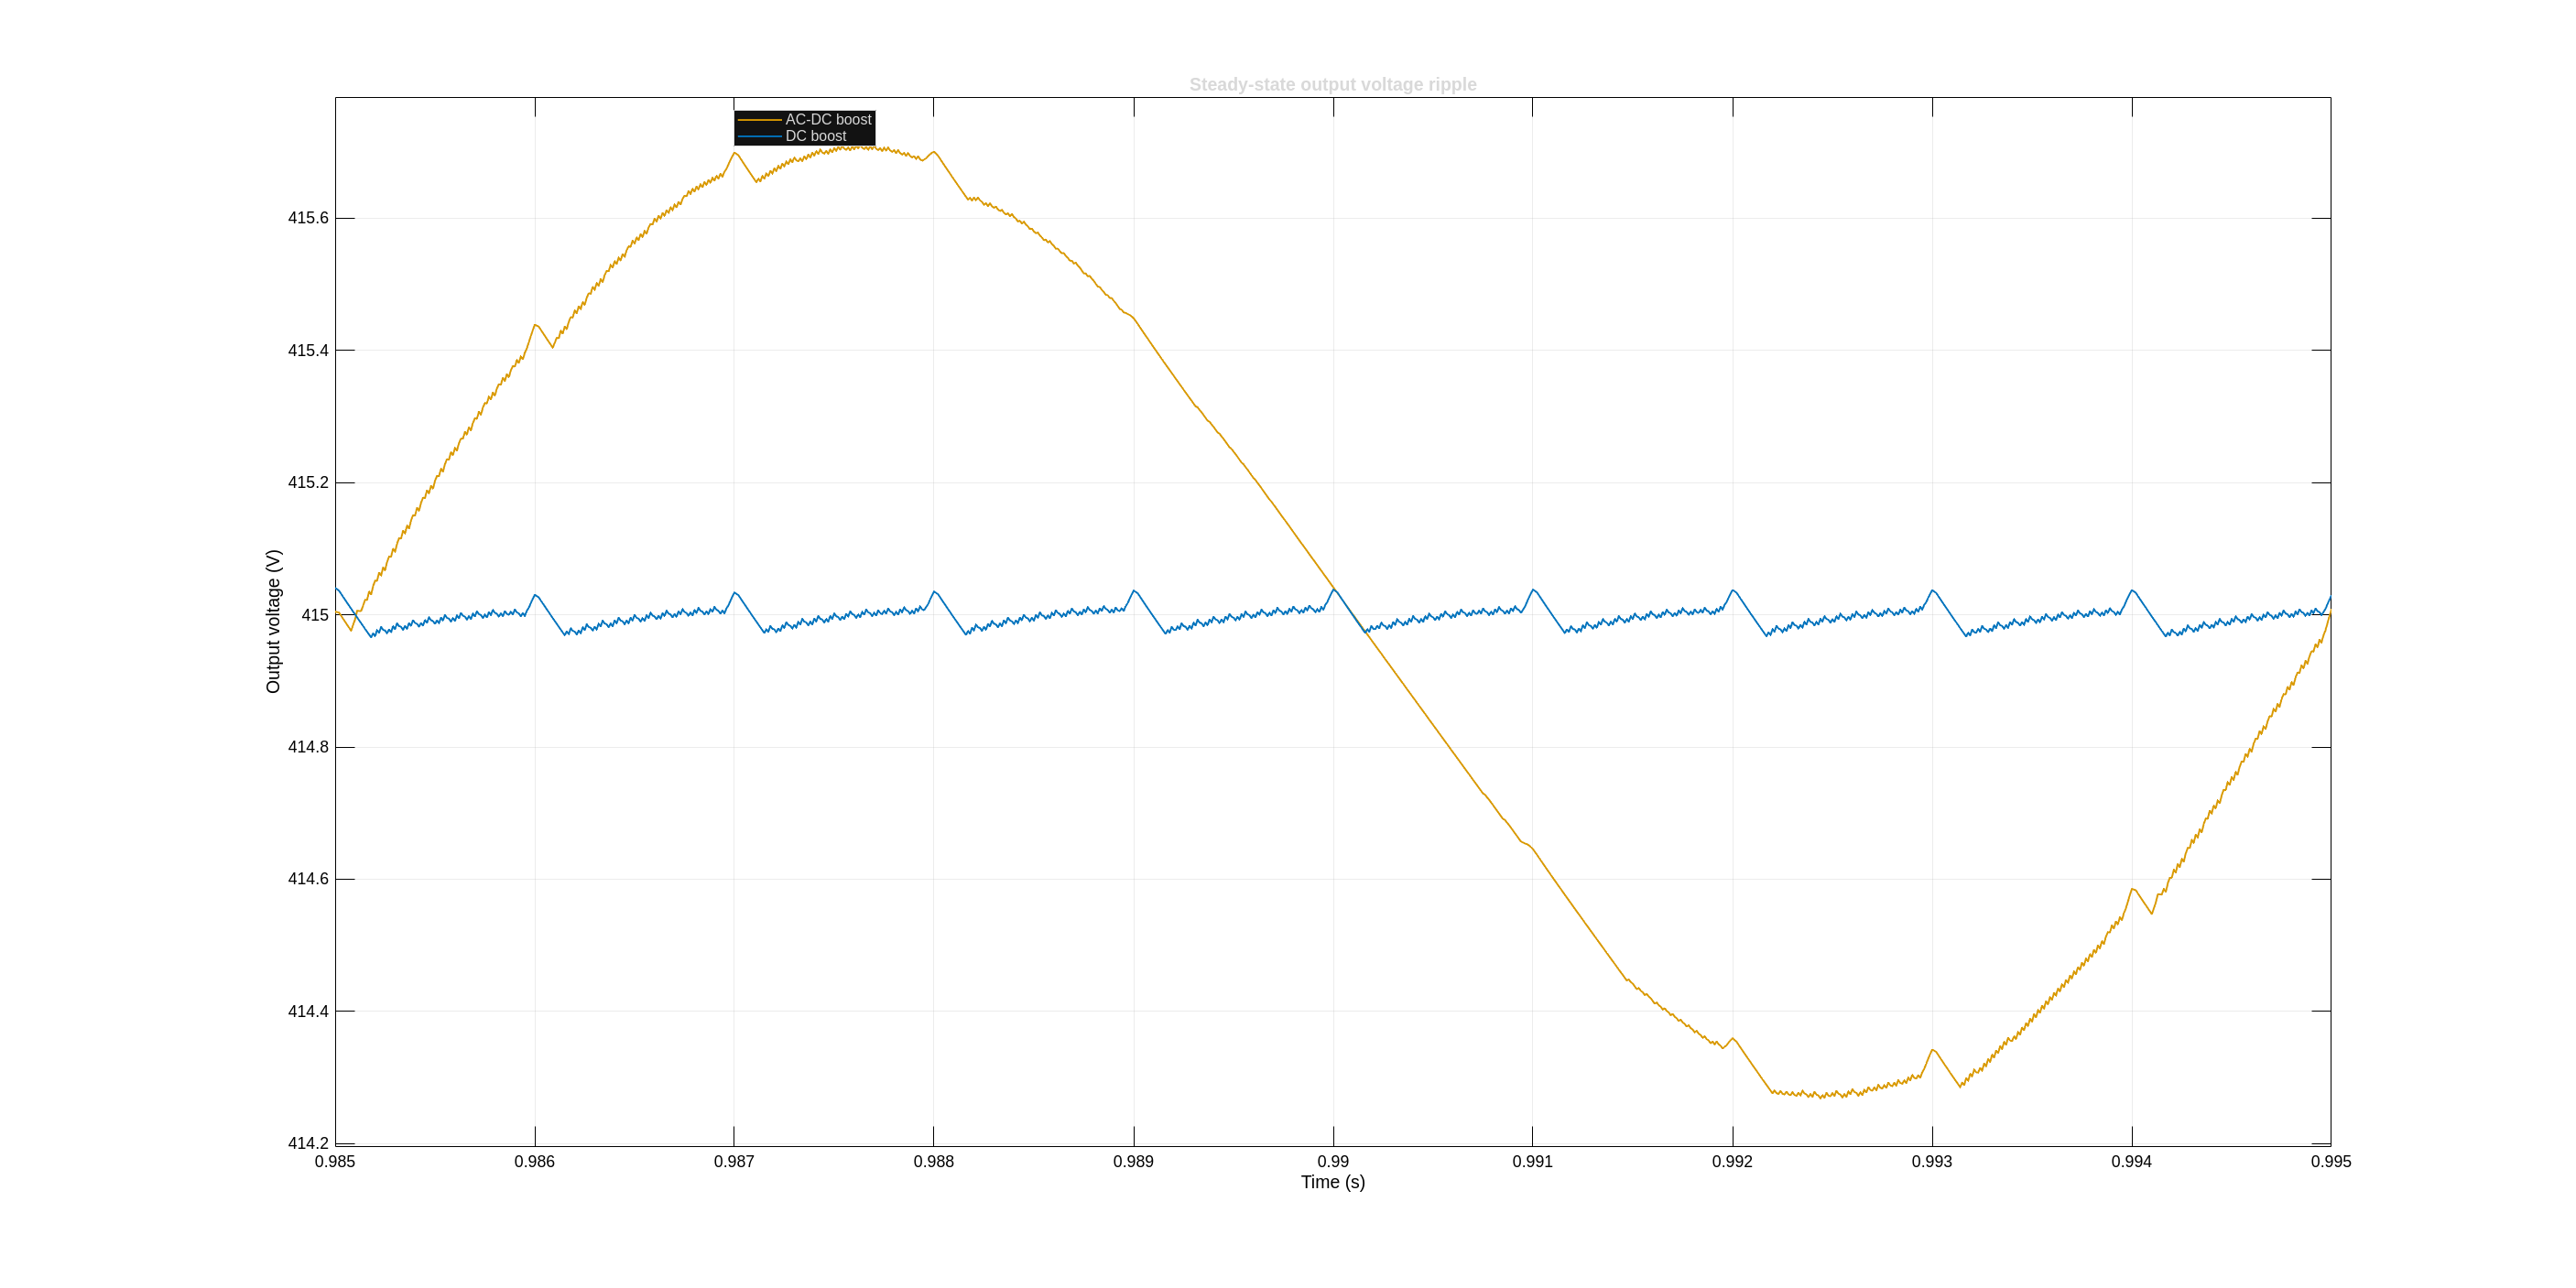
\includegraphics[width=0.92\linewidth]{fig_vout_ripple_zoom.png}
  \caption{Steady-state output voltage: the AC-DC converter swings $\approx1.44\,\mathrm{V}$
  at $100\,\mathrm{Hz}$, the DC converter only shows $1\,\mathrm{kHz}$ switching ripple.}
\end{figure}

\subsection{Input Current and Power Factor}
\begin{table}[htbp]
\centering
\begin{tabular}{|l|c|c|}
\hline
Quantity & AC-DC boost & DC boost \\ \hline
Input current & $17.5\,\mathrm{A}$ peak, line-following & $9.3$--$13.9\,\mathrm{A}$, mean $\approx12\,\mathrm{A}$ \\
THD (to 40th harmonic) & $8.9\,\%$ & n/a \\
Power factor & $0.995$ & n/a \\ \hline
\end{tabular}
\caption{Steady-state input current quality.}
\end{table}

The AC-DC converter draws a current in phase with the input voltage, with flat-topped peaks and
dead zones near the zero crossings (Fig.~\ref{fig:iin}). Despite this, harmonic distortion is
moderate ($8.9\,\%$), giving a power factor of $0.995$. The DC converter draws a sawtooth around
its mean value and has no power-factor concept.

\begin{figure}[htbp]
  \centering
  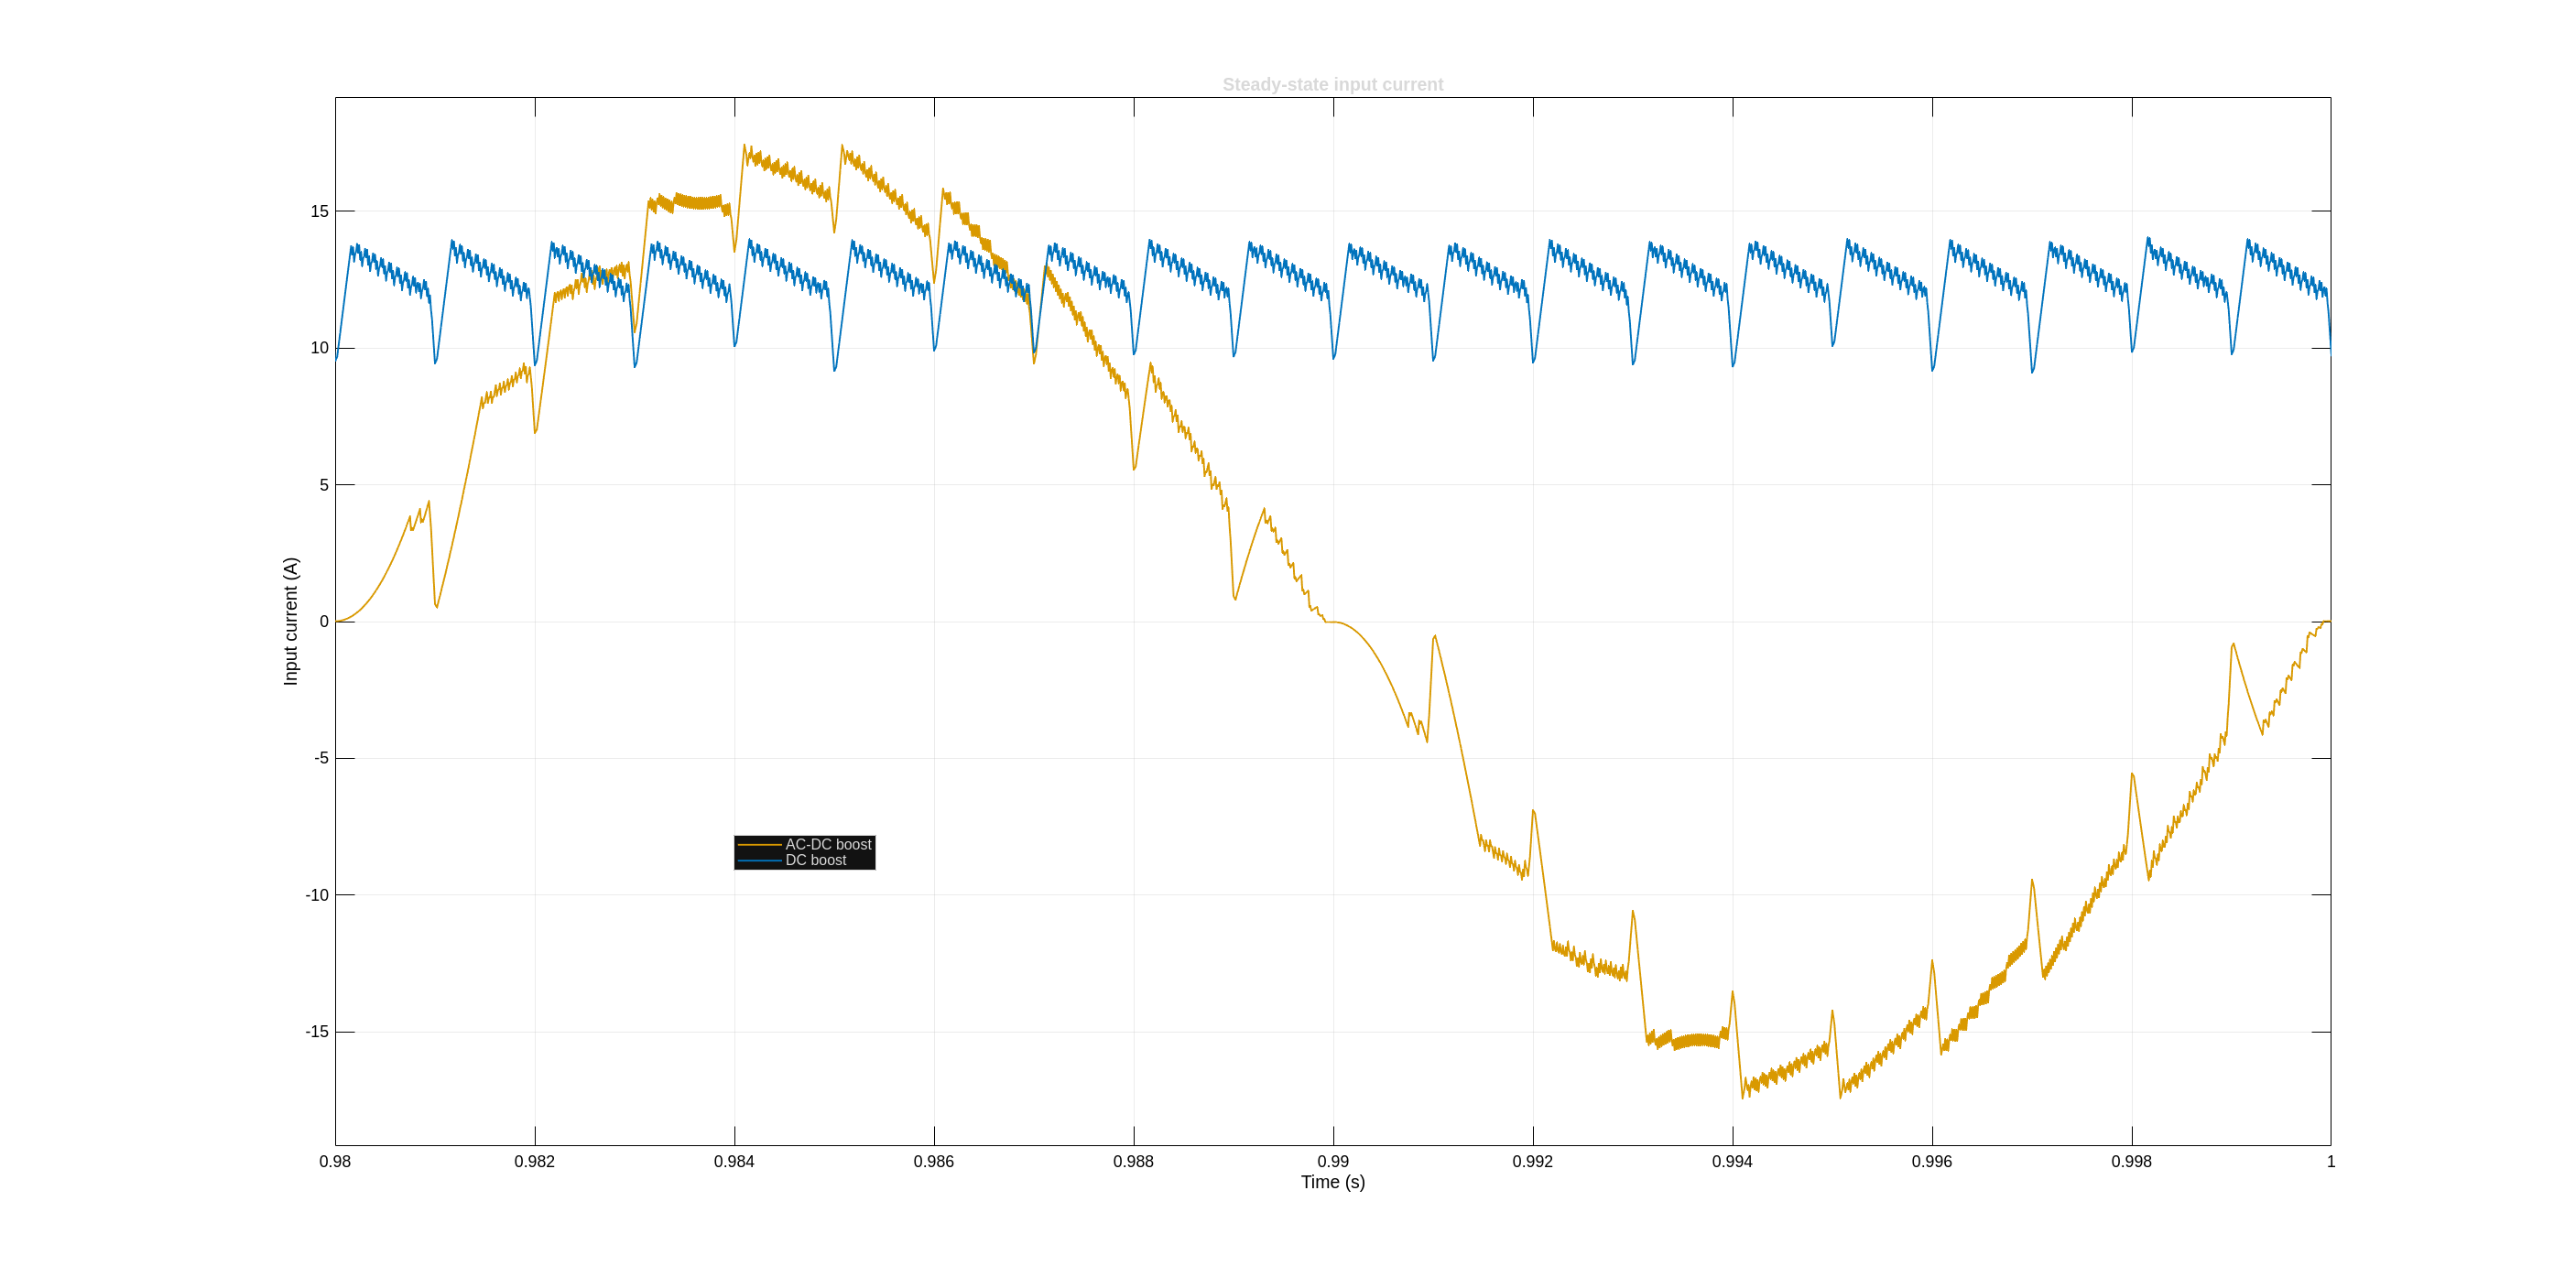
\includegraphics[width=0.92\linewidth]{fig_input_current_zoom.png}
  \caption{Steady-state input current of both converters.}
  \label{fig:iin}
\end{figure}

\section{Discussion}
\begin{itemize}
\item \textbf{Output ripple.} The AC-DC converter pays for its sinusoidal input current with a
  $100\,\mathrm{Hz}$ output ripple about $12\times$ larger than the DC converter's total ripple.
  Since $\Delta V_{pp}\propto1/C$, a larger output capacitor reduces it proportionally.
\item \textbf{Switching ripple.} The AC-DC bench shows about twice the $1\,\mathrm{kHz}$ ripple of the
  DC bench. A likely contributor is that its duty cycle rises towards one near each zero crossing,
  while the DC bench holds an almost constant duty; this was not separately verified.
\item \textbf{PFC quality.} At $1\,\mathrm{kHz}$ there are only 20 switching cycles per line cycle,
  which explains the visible flat tops and dead zones; a higher switching frequency would be
  expected to reduce THD further (not simulated here).
\item \textbf{Startup.} The $\approx205$--$225\,\mathrm{A}$ inrush is inherent to the boost
  topology (the diode conducts before the switch acts) and cannot be removed by the controller; a
  soft-start or pre-charge circuit would be required. Anti-windup clamping, in contrast, removes
  the voltage overshoot entirely and shortens settling from $>1\,\mathrm{s}$ to $<0.5\,\mathrm{s}$.
\item \textbf{Limitations.} Values were read from simulation scopes and a short ten-to-twenty
  cycle window, with ideal components and no parasitics.
\end{itemize}

\section{Conclusion}
For identical power stage, load and control, the DC boost converter achieves far lower output
ripple ($0.12\,\mathrm{V}$ vs.\ $1.45\,\mathrm{V}$ peak-to-peak), while the AC-DC boost converter
delivers the line-side benefit that justifies its ripple: a line-following input current with
$8.9\,\%$ THD and a power factor of $0.995$ at only $1\,\mathrm{kHz}$ switching. Proper anti-windup
is essential for a clean startup in both.

\appendix
\section{Measured Data}
\begin{table}[htbp]
\centering
\small
\begin{tabular}{|p{5.2cm}|p{2.6cm}|p{2.6cm}|p{2.6cm}|}
\hline
Quantity & AC-DC & DC & Source \\ \hline
Output mean & $415\,\mathrm{V}$ & $415\,\mathrm{V}$ & scope \\
Output pk-pk, total ($0.8$--$1.0\,\mathrm{s}$) & $1.454\,\mathrm{V}$ & $0.121\,\mathrm{V}$ & script \\
Output pk-pk, scope zoom & $1.44\,\mathrm{V}$ ($414.27$--$415.71$) & $0.07\,\mathrm{V}$ ($414.97$--$415.04$) & scope readout \\
Switching ripple ($1\,\mathrm{kHz}$) & $0.151\,\mathrm{V}$ & $0.075\,\mathrm{V}$ & script \\
Input current range & $\pm17.5\,\mathrm{A}$ & $9.3$--$13.9\,\mathrm{A}$ & scope \\
THD (40 harmonics) & $8.9\,\%$ & n/a & script \\
Power factor & $0.995$ & n/a & script \\
Inrush current & $\approx225\,\mathrm{A}$ & $\approx205\,\mathrm{A}$ & scope \\
Peak output after inrush & $293\,\mathrm{V}$ & $289\,\mathrm{V}$ & scope \\
Output minimum before switching & $\approx271\,\mathrm{V}$ & $\approx259\,\mathrm{V}$ & scope \\
Start of switching & $\approx0.10\,\mathrm{s}$ & $\approx0.13\,\mathrm{s}$ & scope \\
Current plateau & $\approx36\,\mathrm{A}$ peak & $22\,\mathrm{A}$ & scope \\
Settling to $\pm1\,\%$ & $\approx0.4\,\mathrm{s}$ & $\approx0.45\,\mathrm{s}$ & scope \\ \hline
\end{tabular}
\caption{All numerical results (configuration D).}
\end{table}

\section{Metric Script (\texttt{THDnPF.m})}
Signals were logged from the scopes as \texttt{iscope} (input currents) and \texttt{vscope}
(output and input voltages) in structure-with-time format. Figures were produced with
\texttt{make\_figs.m}.
\begin{verbatim}
get = @(s,k) squeeze(s.signals(k).values);
fs = 1e5;  t = (0.6 : 1/fs : 1.0 - 1/fs)';
i_ac  = interp1(iscope.time, get(iscope,1), t);   % AC input current
v_in  = interp1(vscope.time, get(vscope,2), t);   % AC source voltage
vo_ac = interp1(vscope.time, get(vscope,1), t);
vo_dc = interp1(vscope.time, get(vscope,4), t);

% THD to 40th harmonic; fundamental = bin 21 (20 cycles in window)
N = numel(i_ac);  Y = abs(fft(i_ac))/N*2;
k1 = 21;  h = k1 + (1:39)*20;
THD = sqrt(sum(Y(h).^2)) / Y(k1) * 100;
P  = mean(v_in .* i_ac);
PF = P / (rms(v_in) * rms(i_ac));

w  = t >= 0.8;                       % last 0.2 s = 10 line cycles
pp = @(x) max(x(w)) - min(x(w));
sw = @(x) pp(x - movmean(x, 100));   % removes anything slower than 1 ms
fprintf('THD = %.1f %%, PF = %.3f\n', THD, PF);
fprintf('Vout pk-pk: AC %.3f V, DC %.3f V\n', pp(vo_ac), pp(vo_dc));
fprintf('Switching ripple: AC %.3f V, DC %.3f V\n', sw(vo_ac), sw(vo_dc));
\end{verbatim}

\end{document}
